\documentclass{article}
\usepackage{tikz}

\begin{document}

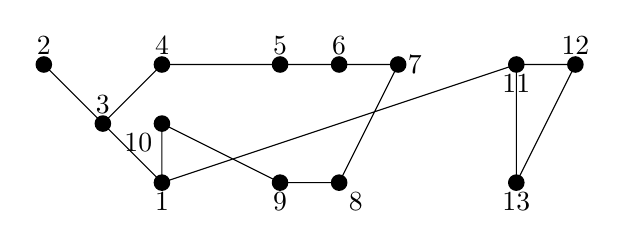
\begin{tikzpicture}[scale=1.5]
    % Define coordinates for each vertex
    \coordinate (1) at (0,0);
    \coordinate (2) at (-1,1);
    \coordinate (3) at (-0.5,0.5);
    \coordinate (4) at (0,1);
    \coordinate (5) at (1,1);
    \coordinate (6) at (1.5,1);
    \coordinate (7) at (2,1);
    \coordinate (8) at (1.5,0);
    \coordinate (9) at (1,0);
    \coordinate (10) at (0,0.5);
    \coordinate (11) at (3,1);
    \coordinate (12) at (3.5,1);
    \coordinate (13) at (3,0);

    % Draw edges between vertices
    \draw (1) -- (2) -- (3) -- (4) -- (5) -- (6) -- (7) -- (8) -- (9) -- (10) -- (1) -- (3) -- (4) -- (5) -- (6) -- (7) -- (8) -- (9) -- (10) -- (1) -- (11) -- (12) -- (13) -- (11);

    % Draw nodes with labels
    \fill (1) circle (2pt) node[below] {1};
    \fill (2) circle (2pt) node[above] {2};
    \fill (3) circle (2pt) node[above] {3};
    \fill (4) circle (2pt) node[above] {4};
    \fill (5) circle (2pt) node[above] {5};
    \fill (6) circle (2pt) node[above] {6};
    \fill (7) circle (2pt) node[right] {7};
    \fill (8) circle (2pt) node[below right] {8};
    \fill (9) circle (2pt) node[below] {9};
    \fill (10) circle (2pt) node[below left] {10};
    \fill (11) circle (2pt) node[below] {11};
    \fill (12) circle (2pt) node[above] {12};
    \fill (13) circle (2pt) node[below] {13};

    % Optional: Add labels to the edges if needed
    % \draw (1) -- node[left] {} (2);
    % \draw (2) -- node[left] {} (3);
    % \draw (3) -- node[left] {} (4);
    % \draw (4) -- node[left] {} (5);
    % \draw (5) -- node[left] {} (6);
    % \draw (6) -- node[left] {} (7);
    % \draw (7) -- node[left] {} (8);
    % \draw (8) -- node[left] {} (9);
    % \draw (9) -- node[left] {} (10);
    % \draw (10) -- node[left] {} (1);
    % \draw (11) -- node[left] {} (12);
    % \draw (12) -- node[left] {} (13);
    % \draw (13) -- node[left] {} (11);
\end{tikzpicture}

\small\sf An outerplanar graph without degree-1 vertices. The triangle $(5,7,9)$ is the only internal cycle, while $(1,2,3)$, $(3,4,5,6,7,8,9,10)$, and $(11,12,13)$ are outer-cycles. A possible cyclic-order is $(1,2,3,4,5,6,7,8,9,10,11,12,13)$.

\end{document}